\chapter{Antecedentes y objetivos}
\label{cap:2-antecedentes}

\section{Antecedentes}

Los algoritmos evolutivos toman como guía la evolución biológica y la llevan al campo de la optimización. A diferencia de otros métodos, esta clase de algoritmos busca ofrecer mejores resultados mediante la evolución de los individuos de una población, haciéndolos mutar, combinando características entre ellos y seleccionando los mejores candidatos a optar a solución de un problema~\cite{eiben_introduction_2003} (normalmente, de optimización no lineal con un amplio espacio de búsqueda), donde otros algoritmos tardarían demasiado o serían directamente inviables.

Este tipo de algoritmos se componen de varios elementos:

\begin{itemize}
    \item \textit{Representación.} Es la manera en que representamos los individuos. Para el caso que aquí nos atañe, un individuo es una intersección vial con un conjunto de semáforos. La duración de cada una de las fases de esos semáforos, así como los retardos, se representan como un vector de números. Cada individuo es una posible solución.
    \item \textit{Función de evaluación (fitness).} Devuelve un valor, a partir de un individuo, que determina qué tan bueno es como solución al problema.
    \item \textit{Población}. Conjunto de individuos. Es útil para determinar cuantos individuos vamos a forzar a competir entre sí en una generación.
    \item \textit{Mecanismo de selección de padres.} Se corresponde con los criterios tenidos en cuenta a la hora de determinar cuáles queremos que sean los individuos que se reproducirán en la generación, normalmente de carácter estocástico.
    \item \textit{Operadores (recombinación y mutación).} Determinan la manera en que se alteran los individuos de la población.
    \item \textit{Mecanismo de selección de supervivientes (reemplazo).} Es similar al mecanismo de selección de padres, pero se realiza en una fase distinta del algoritmo; normalmente después de seleccionar a los padres y son escogidos según el valor que haya devuelto la función de evaluación, pero no es el único criterio.
    \item \textit{Inicialización y terminación.} Finalmente, debemos determinar de qué manera queremos iniciar el algoritmo (normalmente, con individuos generados aleatoriamente) y cómo queremos terminarlo (por ejemplo, tras un número determinado de iteraciones, o en función de un umbral, tomando como guía el \textit{fitness} o la diversidad entre individuos).
\end{itemize}

Esta clase de algoritmos resultan útiles para afrontar el problema de la planificación de la duración de las fases de los semáforos, más conocido como el {Traffic Light Scheduling Problem} (TLSP). Este problema de optimización plantea cuánto deberían durar las fases de los semáforos de uno o varios cruces para mejorar la circulación con respecto a varios parámetros; el más habitual de ellos siendo el tiempo medio de viaje de un grupo de vehículos desde un origen hasta el destino. Otros parámetros, como la distancia media o la contaminación de los vehículos también pueden ser tenidos en cuenta a la hora de evaluar el comportamiento de las distintas configuraciones semafóricas. 

Este tipo de parámetros se pueden emplear en la función de evaluación del algoritmo evolutivo para calcular el valor que correspondería a un individuo; en este caso, un conjunto de semáforos. En el siguiente capítulo se detallarán los parámetros tenidos en cuenta en dicha función, así como otros aspectos relevantes relacionados con el planteamiento del problema.

Para obtener estos valores, es necesario simular el comportamiento de los vehículos con las distintas configuraciones de semáforos. Para esto, se ha empleado SUMO, un simulador de tráfico microscópico de código abierto, que nos proveerá con los parámetros necesarios para la función de evaluación.

La obtención de los datos necesarios para realizar las simulaciones, como el mapa de la localización que queremos simular, así como los datos de los vehículos, han sido obtenidos: de un lado, de OpenStreetMap (para el caso del mapa); y de otro, del Cabildo de Tenerife (para el caso de los datos de circulación de la zona en cuestión). De esto se hablará con extensión en los siguientes capítulos, pues el tratamiento de estos datos conforma la mayor parte del proyecto.

La zona seleccionada para llevar a cabo la simulación ha sido la de la glorieta del Brasil (más conocida como la rotonda del Padre Anchieta), sita en San Cristóbal de La Laguna. La elección de esta zona en particular viene determinada por la gran cantidad de tráfico que absorbe cada día, al estar situada en el corazón del municipio, al haber una gran variedad de viviendas, comercios y lugares de trabajo en las zonas conexas, así como por la presencia de dos campus universitarios pertenecientes a la Universidad de La Laguna. La rotonda no tiene semáforos, por lo cual en este proyecto se han planteado varias configuraciones semafóricas.

Por tanto, lo que se plantea en este proyecto es la obtención de una instancia real, con datos de tráfico incluidos, de la rotonda del Padre Anchieta. Los resultados de la simulación del tráfico realizada por SUMO en dicha instancia servirán de entrada a un algoritmo evolutivo para evaluar si incluyendo semáforos en la rotonda y optimizando la duración de las fases, es posible mejorar la circulación en función de los parámetros especificados.

\subsection{Trabajos previos relacionados}

El planteamiento aquí propuesto ya ha sido tratado desde distintas perspectivas por otros autores en los que se basa este TFG, de entre los que cabe resaltar a:

\begin{itemize}
    \item Segredo \textit{et al.}~\cite{segredo_optimising_2019}. El artículo versa sobre el TLSP y el empleo de varios optimizadores mono y multi-objetivos basados en la diversidad, por ser mucho más eficientes y, en consecuencia, ser capaces de lidiar con zonas significativamente más grandes de ciudades como Berlín, París, Estocolmo o Málaga, en vez de unas pocas intersecciones, llegando a simular casi 1000 de estas y más de 2600 vehículos.
    \item Sánchez \textit{et al.}~\cite{sanchez_applying_2008}. El artículo, de 2008, versa también sobre el TLSP pero aplicado a las Ramblas, en Santa Cruz de Tenerife. El autor, con la optimización propuesta de las duraciones de las fases de los semáforos, consigue mejoras notables en la circulación del tráfico.
    \item Dorta Acosta~\cite{dorta_acosta_simulacion_2019}. En este caso se trata de un TFG de un compañero de la Escuela, que versa sobre la instalación de semáforos inteligentes en la rotonda de Padre Anchieta.
\end{itemize}


\section{Objetivos}

Con la elaboración de este proyecto lo que se propone es la instalación de semáforos en la rotonda, cuyas duraciones de fase han sido optimizadas mediante un algoritmo evolutivo, para comprobar si con la instalación de estos semáforos es posible mejorar la circulación del tráfico en función de determinados parámetros como la duración media de los trayectos de los vehículos, la velocidad media, la cantidad de vehículos que han logrado completar su trayecto en una hora, etc.

\begin{figure}[ht]
    \centering
    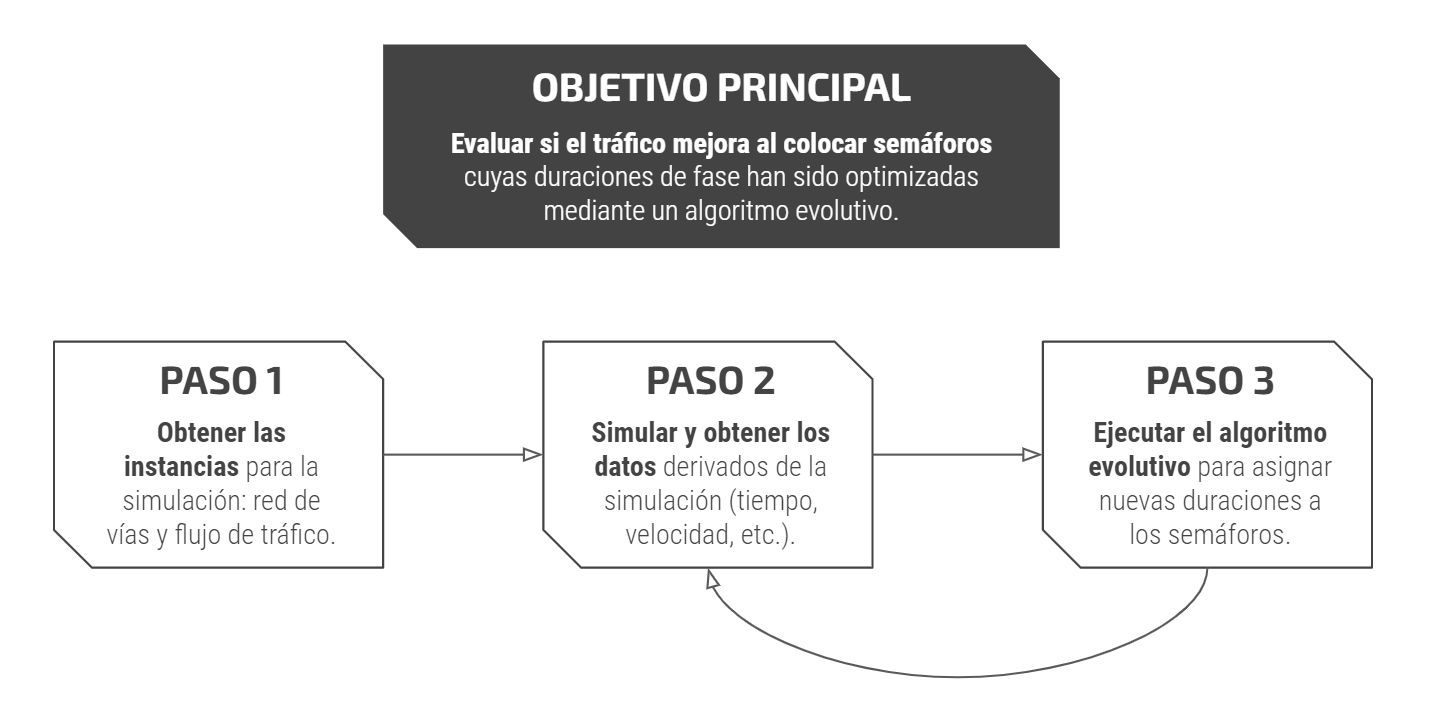
\includegraphics[width=\textwidth]{report/images/evolutionary_alg_graph.png}
    \caption{Gráfica del proceso general del trabajo.}
    \label{fig:evolutionary_alg_graph}
\end{figure}

En comparación con las medidas antes mencionadas, la que se propone supone un coste considerablemente más bajo, no molestaría tanto a los conductores durante la instalación (la cual sería también mucho más corta y sencilla) y que plantea un problema muy interesante que podría ser reaprovechado para otras vías sin coste alguno (si ya tuvieran semáforos instalados).

Para llevar a cabo el proyecto, se han empleado principalmente dos herramientas.

\begin{itemize}
    \item La primera de ellas es SUMO~\cite{lopez_microscopic_2018}, un simulador de tráfico microscópico que nos permitirá evaluar cómo se comporta el tráfico en la rotonda de Padre Anchieta, con datos de tráfico provistos por el Cabildo de Tenerife.
    \item La segunda es Genetics.js~\cite{abrante_dorta_framework_2019}, una librería orientada a algoritmos evolutivos (en particular, algoritmos genéticos) programada en TypeScript.
\end{itemize}
